% This work is licensed under the Creative Commons Attribution-NonCommercial 4.0 International License.
% To view a copy of this license, visit http://creativecommons.org/licenses/by-nc/4.0/
% or send a letter to Creative Commons, PO Box 1866, Mountain View, CA 94042, USA.

% !TEX TS-program = xelatex

\documentclass[../Main/chem371-notes.tex]{subfiles}

\setcounter{chapter}{3}
\begin{document}

\chapter{Basis Sets}

In the previous chapter we introduced the Hartree--Fock method. 
The goal of this chapter is to discuss some practical aspects of how Hartree--Fock computations actually run on a computer and the way the are approximated.
We will encounter the idea of using a linear combination of basis functions to approximate the orbitals $\varphi(\mathbf{r})$ in systematically improvable way.
Lastly, we will look at some applications of these ideas.

\section{Exact solutions to the Schr\"{o}dinger equation for the hydrogen atom}
As it was mentioned earlier, we know exact solutions of the Schr\"{o}dinger only for a handful of models.
An example that should be familiar to you is the hydrogen atom.
For this system, the solutions are known to depend on three quantum numbers $n$, $l$, and $m_l$, and that the energy levels (eigenvalues) are given by (in atomic units)
\begin{iequation}
E_n = - \frac{1}{2 n^2}  \, E_\mathrm{h}, \quad n = 1, 2, \ldots
\end{iequation}
The wave function $\psi_{nlm_l}$ is usually expressed in \emph{spherical coordinates} ($r, \theta, \phi$)\mnote{
If you are curious, spherical coordinates are connected to Cartesian coordinates via the following equations
\begin{align*}
x & =  r \sin \theta \cos \phi, \\
y & =  r \sin \theta \sin \phi, \\
z & =  r \cos \theta
\end{align*}
\centering{
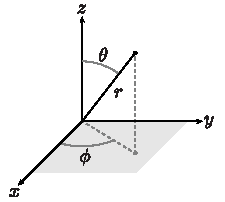
\includegraphics[width=2.0in]{img/spherical_coordinates.pdf}}
\captionof{figure}{Definition of the spherical coordinates $r$, $\theta$, and $\phi$.}
\label{fig:rigidrotor:spherical}
}
 as a product of a function that depends on the electron distance $R_{nl}(r)$ and a term that depends on the angles $\theta$ and $\phi$, which we write as $Y_l^{m_l}(\theta,\phi)$
\begin{equation}
\psi_{nlm_l}(r,\theta,\phi) = R_{nl}(r) Y_l^{m_l}(\theta,\phi)
\end{equation}
For example, the wave function for the  ground state of hydrogen, the 1s orbital, is given by
\begin{equation}
\mathrm{1s} = \psi_{1,0,0}(r,\theta,\phi) = R_{1,0}(r) Y_0^0(\theta,\phi) = 2 e^{-r} \frac{1}{\sqrt{4\pi}} = \frac{1}{\sqrt{\pi}} e^{-r}
\end{equation}
while the 2p$_{z}$ orbital is given by
\begin{align}
\mathrm{2p}_{z} &= \psi_{2,1,0}(r,\theta,\phi) = R_{2,1}(r) Y_1^{0}(\theta,\phi) =
\frac{1}{4\sqrt{2 \pi}}   r e^{-r/2} \cos \theta.
\end{align}

When we turn to more complicated systems, like atoms with more than one electron and molecules, the Schr\"{o}dinger equation becomes intractable and we have to turn to approximate numerical methods to solve it (recall Dirac's quote on this point).
This is what we will look into in the next section.

\section{Bases, basis vectors, and basis functions}

\mfigure{
\centering{
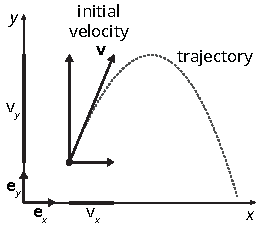
\includegraphics[width=1.75in]{img/trajectory.pdf}}
\captionof{figure}{The trajectory of a particle with initial velocity vector $\mathbf{v} = (v_x, v_y)$.
This vector may be decomposed in the basis of orthogonal unit vectors $\mathbf{e}_x$ and $\mathbf{e}_y$ as $\mathbf{v} = v_x \mathbf{e}_x + v_y \mathbf{e}_y$.}
\label{fig:2dtraj}
}

An important concept when constructing numerical approximations is that of a basis.
To build some intuition about the concept of a basis you can think back to your introductory physics courses and Newton's equations.
Consider the problem of describing the trajectory of a particle under the effect of gravity.
To solve this problem you need to specify the position and initial velocity of the particle.
The position can be specified by the $x$ and $y$ coordinates, and the initial velocity by the velocity in $x$ and $y$ directions ($v_x, v_y$).
These quantities are essentially vectors, which we indicate with the symbols $\mathbf{r} = (x,y)$ and $\mathbf{v} = (v_x,v_y)$. For example, the velocity vector $\mathbf{v}$ can be expressed as a sum of a component pointing in the $x$ direction ($\mathbf{e}_x$) and one pointing in the $y$ direction ($\mathbf{e}_y$)
\begin{equation}
\mathbf{v} = v_x \mathbf{e}_x + v_y \mathbf{e}_y
\end{equation}
The vectors $\mathbf{e}_x$ and $\mathbf{e}_y$ are called a \emph{basis}, because any vector in two dimensions $\mathbf{a}$ can be written as a sum of coefficients multiplied by the basis vectors
\begin{equation}
\mathbf{a} = a_x \mathbf{e}_x + a_y \mathbf{e}_y
\end{equation}
The vectors $\mathbf{e}_x$ and $\mathbf{e}_y$ have another special property: they are orthogonal, which means that their dot product is zero
\begin{equation}
 \mathbf{e}_x \cdot \mathbf{e}_y = 0.
\end{equation}

In the more general case, the velocity is a three dimensional vector, and must be described as a sum of three terms
\begin{equation}
\mathbf{v} = v_x \mathbf{e}_x + v_y \mathbf{e}_y + v_z \mathbf{e}_z
\end{equation}
Interestingly, this idea can also be extended to functions.
For example, suppose we want to approximate some function $g(x)$.
We could start from choosing two simple functions $f_1(x)$ and $f_2(x)$ and approximate $g(x)$ as
\begin{equation}
\label{eq:fit_simple}
g(x) = c_1 f_1(x) + c_2 f_2(x)
\end{equation}
When ``fitting'' the function $g(x)$ in this way, it is convenient to work with functions that are \emph{orthogonal}.
But how does one define the idea of orthogonality for functions? A natural generalization is the overlap integral ($\braket{f_1 | f_2}$)
\mnote{\vspace{-96pt}

One way to think about this is to discretize the integral as a sum.
The integral of a function $f(x)$ is the limit of $\Delta x \rightarrow 0$ of the sum
\begin{equation*}
\int_a^b dx \, f(x) = \Delta x \sum_{k=1}^{n} f(x_k) 
\end{equation*}
where the points $x_k$ form a grid with spacing $\Delta x$.
The integral of a product of two functions $u^*(x) v(x)$ is then also given by the limit of the following expression
\begin{align*}
\int_a^b dx \, u^*(x) v(x) = \Delta x \sum_{k=1}^{n} u^*(x_k)  v(x_k) 
\end{align*}
If we identify the value of the functions at the points $x_k$ as the components of a vector, for example, $v(x_1) = v_1, v(x_2) = v_2, \ldots$, then the above expression can be written as 
\begin{equation*}
\int_a^b dx \, u^*(x) v(x) = \Delta x [u_1 v_1 + u_2 v_2 + \ldots]
\end{equation*}
This looks very similar to the definition of the dot product of two vectors of arbitrary dimension ($\mathbf{u} \cdot \mathbf{v} = u_1 v_1 + u_2 v_2 + \ldots$).
}
\begin{equation}
\text{``}f_1 \cdot f_2\text{''} = \braket{f_1 | f_2} = \int_{-\infty}^{\infty} dx \, f_1^*(x) f_2(x)
\end{equation}
From this definition, we define two functions to be orthogonal if their inner product is null, $\braket{f_1 | f_2}  = 0$.
 
\section{Approximate solutions via expansion in a basis}
We can now look into how the idea discussed in the previous section can be applied to approximate solutions of the Schr\"{o}dinger equation.
The main point is to use a \emph{linear combination of basis functions}\mnote{
A linear combination of some functions/vectors/etc. ($f_i$) is a sum
\begin{equation*}
f_1 c_1 + f_2 c_2 + \ldots + f_K c_K
\end{equation*}
where the quantities $c_1, c_2, \ldots$ are numbers (they can be real or complex).
} to approximate the wave function.
This is a very common strategy for studying differential equations that are too difficult to solve in analytical form.
In Eq.~\eqref{eq:fit_simple} we considered the case of a basis composed by two functions.
However, in the more general case, we approximate $g(x)$ as a sum of a finite number ($K$) of fixed functions $f_i(x)$, called basis functions.
Each basis function is multiplied by the coefficients $c_i$ and the approximation is given by
\begin{equation}
g(x) \approx  c_1 f_1(x) +  c_2 f_2(x) + \cdots + c_K f_K(x) = \sum_{i=1}^{K} c_i f_i(x) 
\end{equation}
\mfigure{\\
\centering{
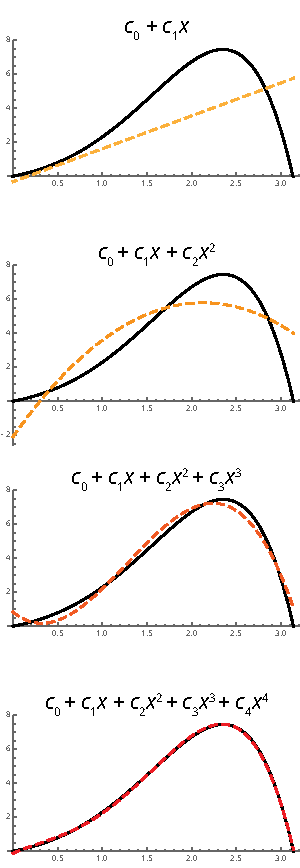
\includegraphics[width=1.75in]{img/basis_expansion.pdf}
}
\captionof{figure}{Example of expansion of the function $\exp(x) \sin(x)$ in a basis of polynomials $x^i$.
By the time we include fourth powers of $x$ this function is approximated well in the entire range $0 \leq x \leq \pi$.}
\label{fig:fit}
}
You can think of this approximation as fitting the function $g(x)$ with the basis functions, where the unknowns are the fitting coefficients $c_i$.
An important point is that, if the basis $\{ f_i(x) \}$ is chosen judiciously, the approximate solution should converge to the exact $g(x)$ when the number of basis functions ($K$) is increased.

This process is illustrated in Fig.~{fig:fit}, where the function $\exp(x) \sin(x)$ is approximated with a basis of polynomials of $x$.
In this example, we stop at the polynomial of order $K$ (here we also include the constant term $x^0 = 1$)
\begin{equation}
g(x) \approx  c_0 +  c_1 x + \cdots + c_K x^{K} = \sum_{i=0}^{K} c_i x^{i}
\end{equation}
As you can see, the first two approximations are not very good, and by the time we use a forth-order polynomial we cannot easily distinguish $\exp(x) \sin(x)$ from its approximation.

\section{Gaussian atomic orbitals bases}

To understand how we use bases in quantum chemistry we will start by learning how atomic orbitals are approximated with a Gaussian basis.
Since the early days of computational chemistry it has become common practice to approximate atomic orbitals using a basis of \emph{Gaussian functions}.
For example, if we want to approximate the 1s orbital of the hydrogen atom, $\mathrm{1s}=  \frac{1}{\sqrt{\pi}} e^{-r}$, an expansion in Gaussian functions consists of the following approximation
\begin{equation}
\frac{1}{\sqrt{\pi}} e^{-r} \approx \sum_\mu C_\mu \exp(- \alpha_\mu r^2)
\end{equation}

At this point we should ask: \emph{Why would we want to approximate a function that we already know how to write in closed form?}
The answer is that all quantum chemistry methods need to know integrals of atomic orbitals like
\begin{equation}
\int d\mathbf{r}_1 \, d\mathbf{r}_2 \, \frac{\phi^*_i(\mathbf{r}_1) \phi^*_j(\mathbf{r}_2) \phi_k(\mathbf{r}_1) \phi_l(\mathbf{r}_2)}{r_{12}}
\end{equation}
These integrals are difficult to compute with function of the form $e^{-\alpha r}$, but they turn out to be doable if one instead uses functions of the form $\exp(- \alpha r^2)$.\mnote{This is due to the Gaussian product theorem, which states that the product of two multidimensional Gaussians is still a Gaussian function.}

For each type of atomic orbital (s, p, d, etc.) one can write a corresponding Gaussian orbital obtained by multiplying a 3D spherical Gaussian function $\exp(-\alpha r^2)$ times a polynomial in the coordinates $x$, $y$, and $z$
\begin{equation}
\label{eq:primitive}
x^l y^m z^n e^{-\alpha r^2}
\end{equation}
As we have seen, s orbitals are obtained from a combination of Gaussians
\begin{equation}
e^{-\alpha r^2}
\end{equation}
while p orbitals can be represented with a product of $x$, $y$, or $z$ and a Gaussian
\begin{equation}
x e^{-\alpha r^2}, y e^{-\alpha r^2}, z e^{-\alpha r^2}
\end{equation}
Atomic orbitals of d type can be formed by quadratic polynomials times a Gaussian.
In this case there are six combinations
\begin{equation}
x^2 e^{-\alpha r^2}, y^2 e^{-\alpha r^2}, z^2 e^{-\alpha r^2},
xy e^{-\alpha r^2}, yz e^{-\alpha r^2}, xz e^{-\alpha r^2}
\end{equation}
We call these d orbitals \emph{Cartesian Gaussians}, to distinguish them from \emph{spherical Gaussians}, the \emph{five} atomic d orbitals that are obtained when we solve the Schr\"{o}dinger equation.
In a quantum chemistry code, integrals are first computed using Cartesian Gaussians and then these are combined to form spherical Gaussians.

The Gaussians functions defined in Eq.~\eqref{eq:primitive} are called \emph{primitives}. To represent the correct shape of atomic orbitals several primitives are combined together using a fixed set of coefficients to form numerically accurate approximations to atomic orbitals.
\begin{equation}
\chi_\mu(\mathbf{r})
\end{equation}


\section{The linear combination of atomic orbitals approximation}
A sensible choice for approximating the shape of orbitals is to use a basis that is as close as possible to the atomic orbitals of isolated atoms.
The intuition here is that a lot of the details of the structure of atoms is preserved in molecules.
So it makes sense to use atomic orbitals as building blocks for approximating molecular orbitals.
This idea is called the \emph{linear combination of atomic orbitals} (LCAO), which you have already encountered when you applied molecular orbital theory to simple molecules like \ce{H2}, where the bonding orbital is the in-phase combination (superposition) of two 1s atomic orbitals, or when you were introduced to the concept of hybrid orbitals like the \ce{sp^3} hybrids of carbon in methane.
This is not the only way quantum chemistry computations are done,\mnote{Other examples include using plane waves [$\exp(i \mathbf{k} \cdot \mathbf{r})$] and numerical grids to approximate the orbitals.} but it is by far the most common approach used in most quantum chemistry programs.

%In principle, the best way to implement the LCAO approximation is to use atomic orbitals from very precise computations.
%However, this is an impractical approach because some of the integrals that are required in Hartree--Fock theory and more advanced methods cannot be efficiently computed using 




\centering{
\captionof{table}{Convergence of the energy of the hydrogen atom as a function of the computational basis.
The exact solution corresponds to the analytic solution of the Schr\"{o}dinger equation.}
\begin{tabular}{@{} cccc @{}} % Column formatting, @{} suppresses leading/trailing space
\toprule
Basis    & Basis Functions & Energy (\Eh) & Error (\Eh) \\
\midrule
cc-pVDZ &   5 & $-$0.499278403 & 0.000721597 \\ 
cc-pVTZ &  14 & $-$0.499809811 & 0.000190189 \\ 
cc-pVQZ &  30 & $-$0.499945569 & 0.000054431 \\ 
cc-pV5Z &  55 & $-$0.499994535 & 0.000005465 \\ 
cc-pV6Z &  91 & $-$0.499999245 & 0.000000755 \\ 
Exact &  $\infty$ & $-$0.500000000 & 0.000000000\\
\bottomrule
\end{tabular}
}

\centering{
\begin{tabular}{@{} ccc @{}} % Column formatting, @{} suppresses leading/trailing space
\toprule
Basis    & Basis Functions & Energy (\Eh) \\
\midrule
cc-pVDZ &  10 & $-$0.600264667 \\
cc-pVTZ &  28 & $-$0.602244426 \\
cc-pVQZ &  60 & $-$0.602520583 \\
cc-pV5Z & 110 & $-$0.602619758 \\
cc-pV6Z & 182 & $-$0.602632085 \\
\bottomrule
\end{tabular}
\captionof{table}{Convergence of the energy of the \ce{H2+} molecule at a bond distance $r_\mathrm{HH}$ = 2 bohr as a function of the computational basis.}
}


\end{document}